\newpage


\section{Przegląd literatury -- SZKIELET POZIOMU 2}
\label{sec:literature}

\subsection{Metody partycjonowania grafów}

1. (PODZIAŁ METOD PARTYCJONOWANIA -OD TYCH NAJMNIEJ WAŻNYCH DO NAJWAŻNIEJSZYCH) Rozbudowany podział metod został zaproponowany przez autorów artykułu - \cite{metis}
oraz \cite{1364754}
Zgodnie z ich analizą metody dzielimy na:
\newline\newline
a. (TUTAJ O METODACH SPEKTRALNYCH) Metody spektralne - partycjonowanie spektralne daje dobre rezultaty i jest metodą w miarę często używaną
\cite{10.1137/0611030, 10.5555/147877.147902, improved_spectral}. Są to jednak metody kosztowne z racji na
obliczanie wektorowa własnego odpowiadającego drugiej najmniejszej wartości własnej (Fielder wektor).
Istnieję udane próby ulepszenia czasu wykonania tych metod, które polegają na liczeniu Fielder wektora poprzez
algorytm wielopoziomowy - MSB \cite{fast_multilevel}. Jednak nawet te metody wciąż charakteryzują się wysoką złożonością.

b. (TUTAJ O REKURSYWNYCH METODACH) Metody rekursywne -
Są to metody często prostsze w implementacji, jednak nie sprawdzają się tak dobrze w kontekście bardziej
skomplikowanych problemów głównie ze względu na to, że mają zachłanną naturę.
Ponadto wykorzystanie takich algorytmów w kontekście niepodzielnych obszarów nie zdaje egzaminu,
ze względu na ich specyfikę. Podejście do partycjonowania zakładające dzielenie grafu na coraz mniejsze
części sprawia, że nie jesteśmy w stanie uwzględniać części niepodzielnych, lub rozwiązanie tego problemu byłoby skomplikowane.
Przykład - dzielimy siatkę na 4 części. Można sobie wyobrazić sytuację, kiedy obszar niepodzielny zajmuje 50\% całej siatki.
Po pierwszej turze rekursywnego algorytmu mamy dwie partycje, każda zajmująca 50\% powierzchni. Chcielibyśmy podzielić
każdą z nich na dwie części, natomiast nie jesteśmy w stanie tego zrobić ponieważ jedna z nich jest w całości obszarem
niepodzielnym.
Metoda \cite{recursive} zakłada żę dzielimy siatkę na liczbę obszarów,
która jest równa potędze liczby dwa. Ta metoda potrafi także dzielić siatkę wedle możliwości obliczeniowych
poszczególnych rdzeni procesora. Czasami metody rekursywne są implementowane jako faza metod
bisekcji spektralnej \cite{10.1137/0611030}.

c. (TUTAJ O METODACH GEOMETRYCZNYCH) Metody geometryczne - inną klasą metod są metody geometryczne \cite{Miller1994ACP, Raghavan93lineand, 185417, MiTeThVa93, NourOmid1987SolvingFE}.
Ich cechą charakterystyczną jest szybki czas wykonania, natomiast gorsze rezultaty podziału.
Najlepsze wyniki spośród wyżej wymienionych metod prezentują \cite{185417, MiTeThVa93}, natomiast z powodu
losowej natury wymagane jest wielokrotne użycie algorytmu (od 5 do 50 razy) aby uzyskać wynik porównywalny
z metodami spektralnymi. Wielokrotnie wywołanie zwiększa czas otrzymywania rezultatu, natomiast jest
on wciąż niższy od metod spektralnych. Metody geometryczne są aplikowalne tylko w przypadku kiedy dostępne
są współrzędne wszystkich wierzchołków w grafie. Dla wielu dziedzin problemów (programowanie liniowe, VLSI),
nie otrzymujemy współrzędnych wraz z grafem. Istnieją algorytmy, które są w stanie obliczyć współrzędne dla
wierzchołków grafu \cite{Chan95geometricspectral} wykorzystując metody spektralne ale są bardzo kosztowne i dominują czas potrzebny
na samo partycjonowanie grafu.
\newline\newline

\begin{wrapfigure}{r}{0.6\textwidth}
    \vspace{-4mm}
    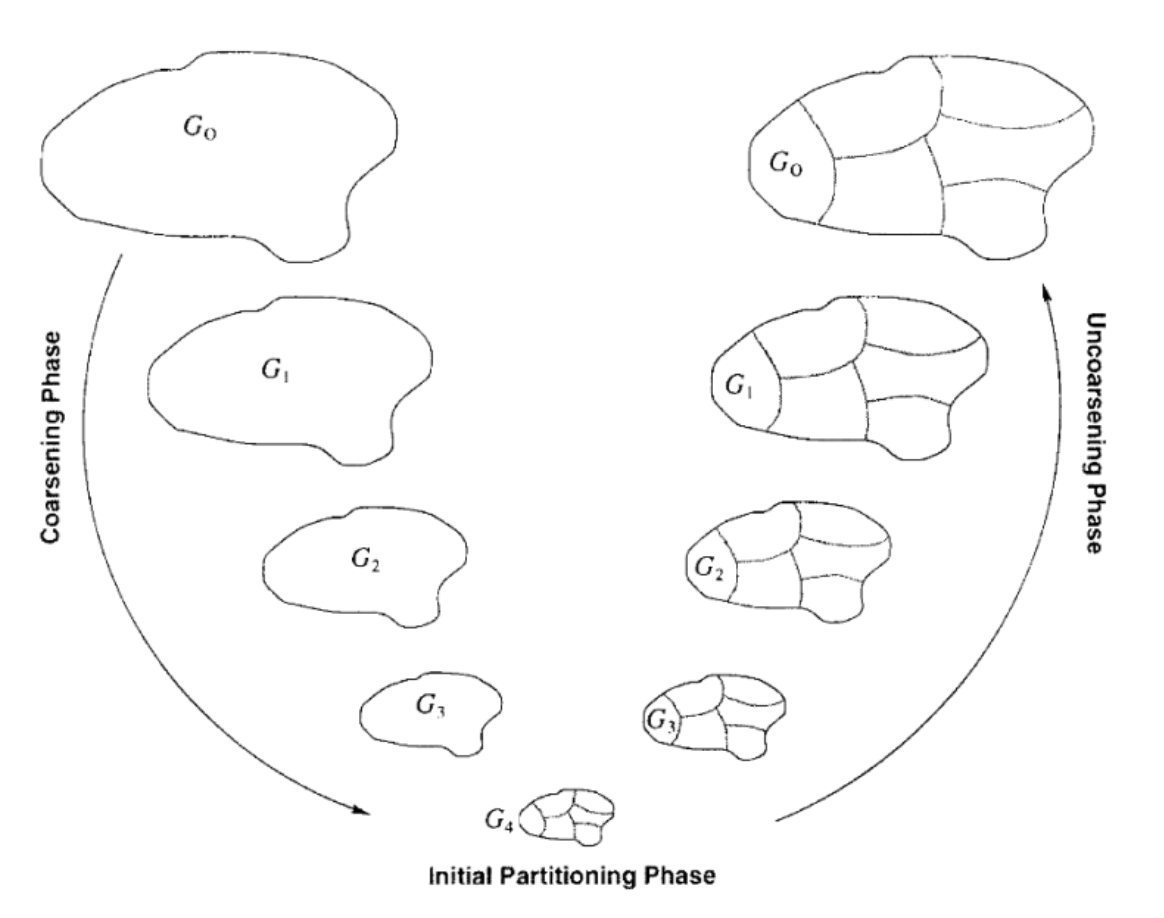
\includegraphics[width=\linewidth]{images/coarsening}
    \caption{Wielopoziomowe partycjonowanie grafu przedstawiające fazę zmniejszania grafu, następnie przypisanie
    partycji na zmniejszonym grafie, na końcu przywrócenie grafu to początkowej wielkości.
    Źródło\cite{KARYPIS199896}.}
    \label{fig:1}
\end{wrapfigure}

d. (TUTAJ O METODACH WIELOPOZIOMOWYCH) Metody wielopoziomowe
\cite{metis, jostle, Bui1993AHF, 103500, 185177, 279334, inproceedings, 129970, 10.1145/165939.165942}
- cechą charakterystyczną tego podejścia jest redukcja
wielkości grafu poprzez łączenie wierzchołków i krawędzi, następnie dzielenie zmniejszonego grafu na partycje, ostatnią fazą
jest przywrócenie początkowego grafu zachowując podział. Często graf zmniejszany jest aż liczba wierzchołków nie osiągnie
liczby partycji, którą chcemy otrzymać \cite{1364754}, a fazie przywracania grafu do początkowej wielkości towarzyszy
algorytm, którego celem jest ulepszanie podziału \cite{article, 10.5555/800263.809204}. Algorytm ten, bazując na zmniejszonym
grafie, niesie za sobą niższy koszt obliczeniowy. Jego działanie polega na zmniejszaniu długości granic pomiędzy partycjami
z jednoczesnym zachowaniem ich wielkości. Na tym etapie może także zostać dodana faza balansowania, która stopniowo zmniejsza różnice
w wielkości pól pomiędzy obszarami. Metody te zostały stworzone z myślą o zmniejszeniu czasu
patrycjonowania kosztem jego jakości. Obecnie dają jednak bardzo dobre rezultaty również w kwestii jakości podziału.
Późniejsze prace w dziedzinie tych algorytmów pokazały, że dają one lepsze rezultaty niż metody spektralne \cite{metis}.
Biblioteki jak Party \cite{1364754}, Metis \cite{metis}, Jostle \cite{jostle}, Chaco \cite{inproceedings},
dające state-of-the-art wyniki w kwestii jakości partycjonowania najczęściej bazują na schemacie wielopoziomowym
\cite{inproceedings}.

\newpage
\subsection{Wybór metody}

\begin{wrapfigure}{r}{0.6\textwidth}
    \vspace{-4mm}
    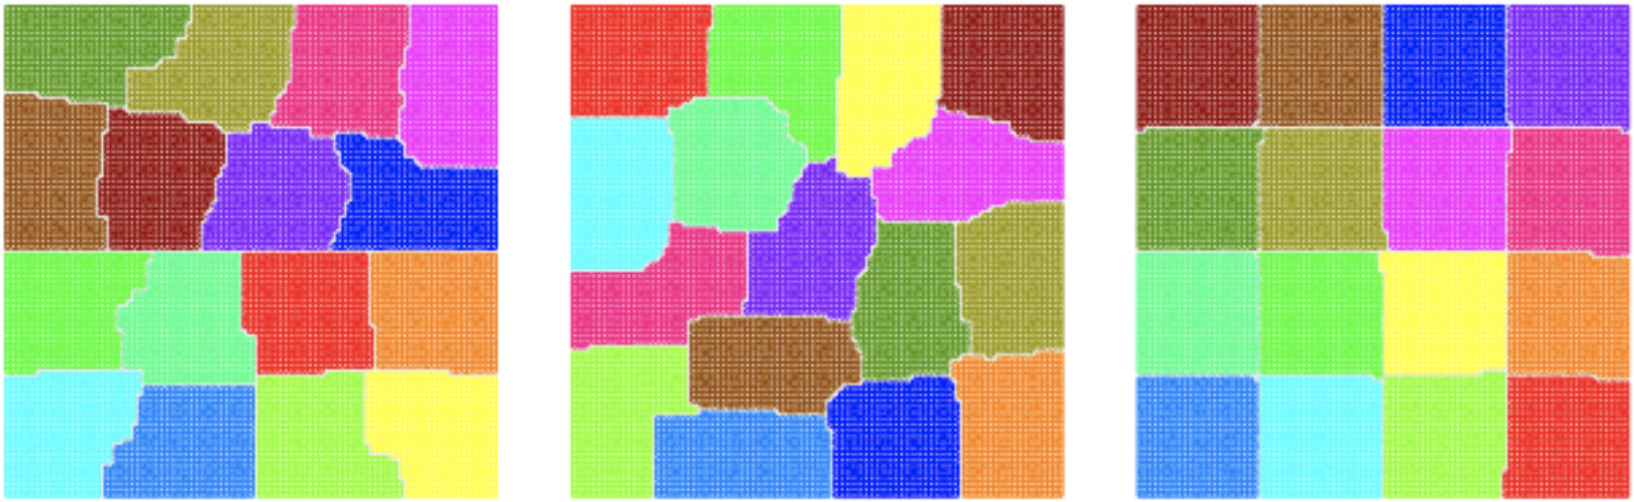
\includegraphics[width=\linewidth]{images/libraries-comparision}
    \caption{Partycjonowanie siatki 100x100 na 16 obszarów. Od lewej - pmetis\cite{metis} uzyskuje edge-cut wynoszący
    688, następnie Jostle\cite{jostle} z wynikiem 695 oraz Party\cite{1364754} z wynikiem 615.}
    \label{fig:test2}
\end{wrapfigure}

(TUTAJ O TYM NA JAKIE PODEJSCIE SIE ZDECYDOWAŁEM I DLACZEGO)

(WSTĘP - UZASADNIENIENIE CZEMU MUSZĘ TWORZYĆ WŁASNĄ METODE NA BAZIE GOTOWYCH METOD)
Wszystkie wyżej wymienione metody nie biorą pod uwagę problemu obszarów niepodzielnych oraz obszarów wyłączonych z obliczeń.
W związku z tym moim zadaniem było znalezienie metody dającej możliwie najlepsze rezultaty w zakresie partycjonowania grafów oraz
dostosowanie jej do wyżej wymienionych rozszerzeń problemu partycjonowania.

(DLACZEGO PARTY - PORÓWNANIE DO INNYCH BIBLIOTEK)
\begin{itemize}
    \item {Metody wielopoziomowe były najlepszym wyborem, z racji na to, że gwarantowały najlepsze wyniki partycjonowania}
    \item {Wiele metod wielopoziomowych do wyboru - \cite{metis, jostle, Bui1993AHF, 103500, 185177, 279334, inproceedings, 129970, 10.1145/165939.165942},
        jednak brałem pod uwagę metody state-of-the-art jak Party \cite{1364754}, Metis \cite{metis}, Jostle \cite{jostle}, Chaco \cite{inproceedings},
        dlatego głównie na nich skupię się w tym porównaniu.}
    \item {podobieństwa i różnice -  Do zmniejszenia grafu stosowane są różne warianty Matching Algorithm.
    Porównanie większości z nich można znaleźć tutaj \cite{Analysis}
    Przykładowo biblioteka Party \cite{1364754} oraz Bui and Jones \cite{Bui1993AHF} stosują Maximal Weighted Matching \cite{weighted_maching}.
    Ze względu na wymagania co do złożoności obliczeniowej wszystkie algorytmy używają heurystyk.
    Wszystkie z tych metod zmniejszają graf, jednak tylko Jostle i Party zmniejsza graf,
    aż do otrzymania liczby wierzchołków równej liczbie partycji, na które chcemy podzielić wejściowy graf.
    Dzięki temu metoda partycjonowania, działająca na najmniejszym możliwym grafie jest dużo prostsza niż w pozostałych metodach.}
\end{itemize}

Biblioteka Party \cite{1364754} okazała się dawać najlepsze rezultaty w porównaniu do innych bibliotek dających rezultaty
state-of-the-art.
Ponadto faza zmniejszania grafu często jest stosunkowo łatwa do zrównoleglenia \cite{KARYPIS199871}. Fazą, która nie podlega
zrównolegleniu jest faza ulepszania istniejącego podziału.
Najczęsciej bazuje ona na metodzie Fiduccia-Mattheysesa \cite{10.5555/800263.809204},
która jest zoptymalizowaną pod kątem czasu działania heurystyką Kerninghan-Lin (KL) \cite{6771089}.



